
\documentclass[letterpaper,11pt]{scrartcl}
\usepackage{graphicx}
\usepackage{fullpage}

\titlehead{Guam Coconut Rhinoceros Project Technical Report}
\title{OrNV Witch's Brew Experiment 1: A Last Ditch Attempt to Find Virus Pathogenetic for the Guam Coconut
Rhinoceros Beetle Genotype}
\author{Aubrey Moore, Ian Iriarte and Roland Quitugua}

\begin{document}

\maketitle

\begin{abstract}
Bioassays of several isolates of Oryctes nudivirus provided by AgriResearch New Zealand failed to result in 
significant pathogenicity for the Guam CRB genotype. In a 'last ditch' attempt we made a 'witches brew' slurry 
containing all frozen dead beetles from previous bioassays plus frozen virus samples in vials. Forty 
adult beetles were forced to swim in the slurry for 30 minutes on January 22, 2015. A control group of
41 beetles were forced to swim in water. Beetles were checked weekly.

By April 10, 2015, mortality of the virus treated beetles (78\%) was significantly greater than that of the
control group (54\%). Treatment mortality corrected for experimental control mortality by Abbott's 
formula was 51\%.
\end{abstract}

\section*{Methods}

Frozen, dead beetles from previous bioassays were added to one liter of water and made into an aqueous slurry
using a blender. Vials containing remnants of virus samples from AgResearch New Zealand were agitated in 500 ml of 
water, and this suspension was added to the blender. The slurry was poured into a small pail and
forty beetles were made to swim in this for thirty minutes. A control group of beetles was made to swim in water for 
thirty minutes.

Beetles were kept in a large container filled with moist, commercially blended steer manure and soil. 
All beetles were checked weekly. Dead beetles were recorded and frozen.

\section*{Analysis}

Data were analyzed using an IPython notebook (file name = 'OrNV.ipynb'). Significance of differences in mortality
were determined using a Fisher's exact test, and final mortality was adjusted using Abbott's formula.

\section*{Results and Discussion}

Cumulative mortality of virus-treated beetles (78\%) on April 10 (Fig. \ref{mortality}) was significantly greater than that of 
control beetles (54\%); (p = 0.0005; Fisher's exact test). Treatment mortality corrected for experimental control mortality by Abbott's 
formula was 51\%.

% FIGURES HERE 
%%%%%%%%%%%%%%
 
\begin{figure}
\centering
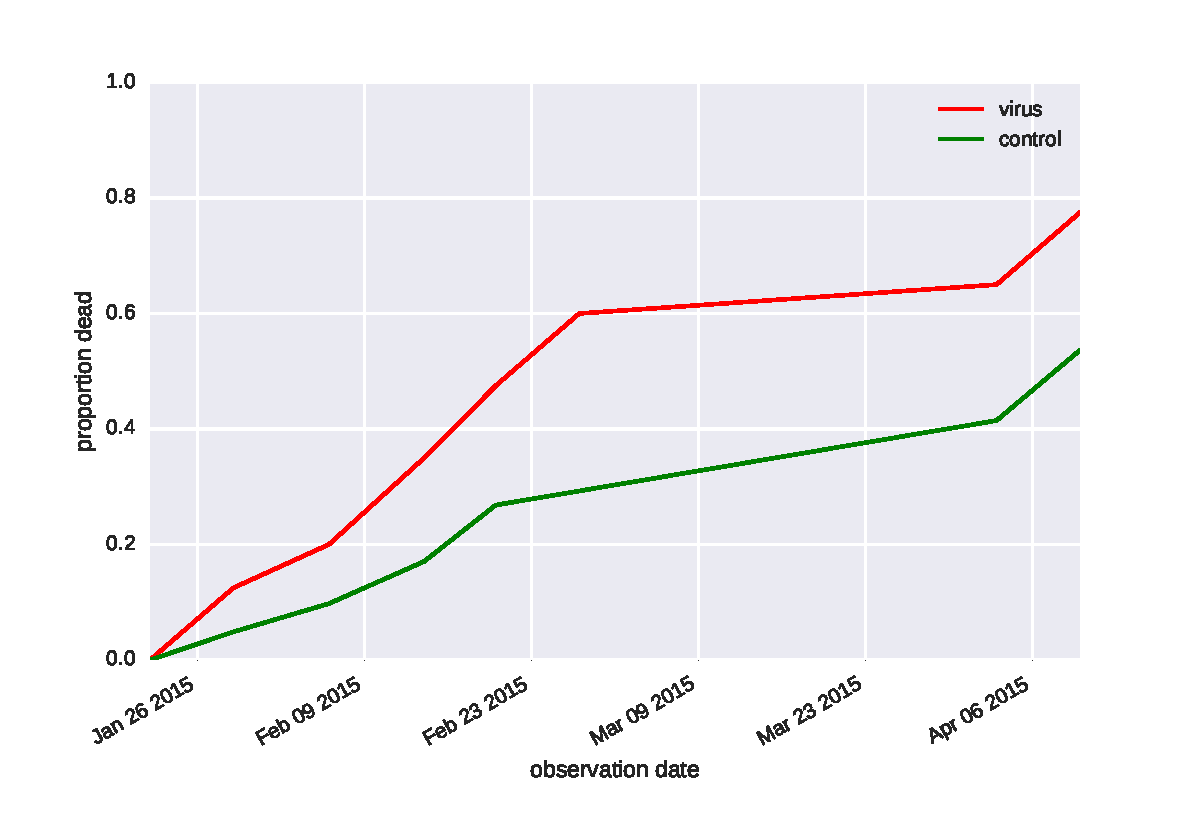
\includegraphics[width = \textwidth]{wb1_mortality.pdf}
\caption{Cumulative mortality.}
\label{mortality}
\end{figure} 
 
% END OF FIGURES
%%%%%%%%%%%%%%%%
 
%\nocite{PER-GRA_2007}
%\bibliographystyle{unsrt}
%\bibliography{ref}

\end{document}